 % Use only LaTeX2e, calling the article.cls class and 12-point type.

\documentclass[12pt]{article}

% Users of the {thebibliography} environment or BibTeX should use the
% scicite.sty package, downloadable from *Science* at
% www.sciencemag.org/about/authors/prep/TeX_help/ .
% This package should properly format in-text
% reference calls and reference-list numbers.

\usepackage{scicite}

% Use times if you have the font installed; otherwise, comment out the
% following line.

\usepackage{times}

\usepackage{enumitem}
\usepackage{float}
\usepackage{graphicx}
\usepackage{subcaption}
\usepackage[table,xcdraw]{xcolor}

% The preamble here sets up a lot of new/revised commands and
% environments.  It's annoying, but please do *not* try to strip these
% out into a separate .sty file (which could lead to the loss of some
% information when we convert the file to other formats).  Instead, keep
% them in the preamble of your main LaTeX source file.


% The following parameters seem to provide a reasonable page setup.

\topmargin 0.0cm
\oddsidemargin 0.2cm
\textwidth 16cm 
\textheight 21cm
\footskip 1.0cm


%The next command sets up an environment for the abstract to your paper.

\newenvironment{sciabstract}{%
\begin{quote} \bf}
{\end{quote}}


% If your reference list includes text notes as well as references,
% include the following line; otherwise, comment it out.

\renewcommand\refname{References and Notes}

% The following lines set up an environment for the last note in the
% reference list, which commonly includes acknowledgments of funding,
% help, etc.  It's intended for users of BibTeX or the {thebibliography}
% environment.  Users who are hand-coding their references at the end
% using a list environment such as {enumerate} can simply add another
% item at the end, and it will be numbered automatically.

\newcounter{lastnote}
\newenvironment{scilastnote}{%
\setcounter{lastnote}{\value{enumiv}}%
\addtocounter{lastnote}{+1}%
\begin{list}%
{\arabic{lastnote}.}
{\setlength{\leftmargin}{.22in}}
{\setlength{\labelsep}{.5em}}}
{\end{list}}


% Include your paper's title here

\title{Réduction Des Couches Convolutives Dans Les Réseaux Profonds} 


% Place the author information here.  Please hand-code the contact
% information and notecalls; do *not* use \footnote commands.  Let the
% author contact information appear immediately below the author names
% as shown.  We would also prefer that you don't change the type-size
% settings shown here.

\author
{Vincent Martineau,$^{1\ast}$\\
\\
\normalsize{$^{1}$Département d'informatique et de génie logiciel, Université Laval, Quebec, Canada}\\
\\
\normalsize{$^\ast$E-mail:  vincent.martineau.1@ulaval.ca.}
}

% Include the date command, but leave its argument blank.

\date{}



%%%%%%%%%%%%%%%%% END OF PREAMBLE %%%%%%%%%%%%%%%%



\begin{document} 

% Double-space the manuscript.

\baselineskip24pt

% Make the title.

\maketitle 



% Place your abstract within the special {sciabstract} environment.

\begin{sciabstract}
  Il y a eu des recherches expliquant comment réduire les couches de convolution dans les réseaux de neurones. Cependant dans les articles proposés les modèles utilisés sont généralement AlexNet et VGG. Lorsqu'essayé sur des réseaux plus complexes tels que ResNet et DenseNet les solutions proposées ne fonctionnent pas. Le but est d'explorer les limites de cette approche et de proposer une solution afin de pouvoir généraliser à des réseaux plus complexes et profonds que ceux dans l'article original de Molchanov. Les expérimentations seront faites sur le transfert de modèle entre ImageNet vers Cifar10 et nous verrons les gains pouvant être faits sur des réseaux profonds. 
\end{sciabstract}



% In setting up this template for *Science* papers, we've used both
% the \section* command and the \paragraph* command for topical
% divisions.  Which you use will of course depend on the type of paper
% you're writing.  Review Articles tend to have displayed headings, for
% which \section* is more appropriate; Research Articles, when they have
% formal topical divisions at all, tend to signal them with bold text
% that runs into the paragraph, for which \paragraph* is the right
% choice.  Either way, use the asterisk (*) modifier, as shown, to
% suppress numbering.

\section*{Introduction}
Les réseaux CNN sont parmi nous depuis très longtemps\cite{lecunn1}. Ces réseaux sont très utilisés dans une grande variété de domaines. Que ce soit avec les systèmes de surveillance, les voitures autonomes ou les appareils intelligents, ce type de réseaux fait maintenant partie de notre quotidien\cite{daily}.

Ces réseaux ont montré qu’ils pouvaient obtenir des résultats excédant les capacités humaines\cite{beathuman}. Dans plusieurs cas, ces modèles sont rendus disponibles au grand public et il est possible de les adapter à des problèmes plus simples pour obtenir de très bons résultats\cite{transfer}. 

\subsection{Description du problèmes}
Afin d'utiliser ces réseaux sûrs de petits appareils, certaines techniques\cite{han1} ont été évalué dans le passé. Plus récemment, un article propose de faire la réduction de filtres de convolution\cite{molchanov}. Cependant l'article se concentre sur les réseaux AlexNet et VGG et ne fonctionne pas sur les réseaux plus complexes présent dans PyTorch\cite{pytorchmodel}.

Le but de cet article sera d'évaluer le travail nécessaire pour pouvoir pousser cette logique vers des réseaux plus complexes tels que ResNet, DenseNet et SqueezeNet. 

\section*{Méthode}
\setcounter{subsection}{0}
La méthode utilisée est une variante de la méthode proposée dans l'article Pruning Convolutional Neural networks for Ressource efficient inference\cite{molchanov}. Le but des modifications est d'étendre les capacités de notre modèle à des réseaux beaucoup plus complexes tels que Res Net, DenseNet et SqueezeNet. 

Voici une liste des étapes à suivre pour obtenir une réduction intéressante: 
\begin{enumerate}[noitemsep, noitemsep]
\item Appliquer le fine tuning sur un réseau pré-entrainé. 
\item Extraire le graphe d'exécution de notre modèle 
\item À partir de notre graphe d'exécution, exclure les couches de convolution que nous ne voulons pas affecter. Ces couches sont détaillées plus tard dans cet article.
\item Réduire les filtres en fonction du critère de réduction. Une description du critère est fournie dans une section futur de cet article. 
\item Réinitialiser l'optimiseur utilisé pour l'entrainement.
\item Appliquer le fine tuning afin de restabiliser le réseau.
\item Recommencer la réduction tant que le réseau ne possède pas la taille voulue. 
\end{enumerate}

Dans cette procédure le critère de sélection est très important pour avoir de bons résultats. Pour cette expérimentation, nous avons utilisé les Taylor Expansions tel que mentionné dans l'article de Molchanov.

Afin de pouvoir exécuter sur des modèles plus complexes, nous avons choisi de ne pas explorer d'autres critères de sélection, mais bien de se concentrer sur l'algorithme nécessaire pour supporter ces modèles. Certains essaies ont aussi été effectué avec l'activation moyenne des filtres et les résultats vont dans la même direction que l'article original.

Une des limitations importante dans notre solution est le besoin de réinitialisé l'optimiseur. Il s'agit d'une restriction majeur de notre proposition et des solutions devront être envisagées.

\subsection{Les couches à ignorer }
Dans la solution proposée, il est important de ne pas appliquer de réduction de filtres juste avant une addition tel que vu dans plusieurs modèles complexes. La figure Figure1 représente cette situation. Le problème dans ce cas est qu’il est nécessaire d’appliquer une réduction équivalente sur toutes les branches entrantes de l'addition. Dans le cas présent, il faudrait donc modifier ce qui vient avant la couche relu et l'entrée de la première convolution du bloc présenté. 

\begin{figure}[H]
	\centering
	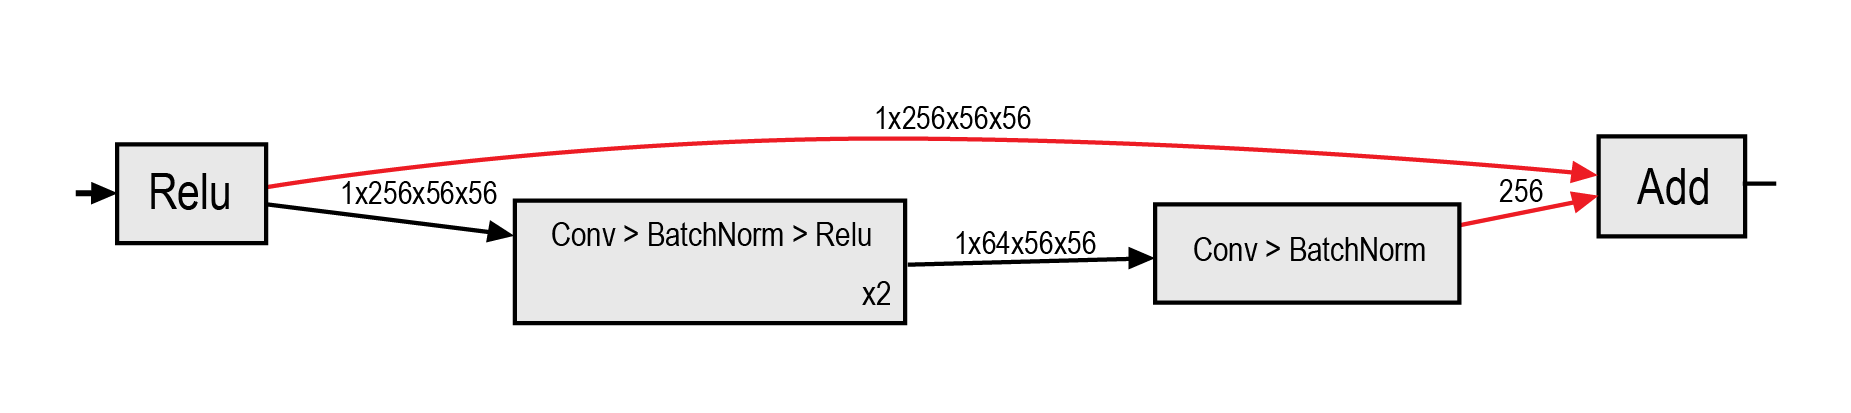
\includegraphics{fig/residual_add}
	\caption{Dans la figure suivante il est impossible de réduire la seconde couche de convolution pour la branche du bas puisqu'il serait aussi nécessaire de modifier la couche précédent ce bloc ResNet pour que la connection résiduelle aie la bonne taille.}
	\label{fig:residualadd}
\end{figure}

Un autre problème potentiel survient lorsqu'une couche est réutilisée. Dans ce cas il faut que l'entrée de notre couche soit compatible avec la sortie de la couche que nous traitons. du coup, nous devons affecter les couches précédentes pour que les dimensions concordent aussi. Ce qui revient au même problème que l'addition.

Il est à noter qu'il est possible qu'il existe un algorithme fiable qui permet de gérer ces cas, mais l'article présent n'explore pas ces options.
Finalement, il est crucial de ne pas affecter une couche si elle influence directement le nombre de sorties du réseau. Une telle pratique affecterait directement la performance et l'entrainement du modèle. Il pourrait y avoir un décalage entre les classes lors de la classification et la fonction de perte pourrait devenir invalide.

\subsection{Pratiques à éviter}
Lors de la construction du modèle, il est très important d’éviter les valeurs fixes lors de l’inférence. Par exemple, dans le modèle AlexNet, il y a le code de la partie gauche de la figure 2 qui nous empêche de réduire la dernière couche de convolution avant la couche pleinement connectée. En effectuant la modification présenté dans la figure 2, il est maintenant possible de réduire cette couche de convolution. 
\begin{figure}[H]
	\centering
	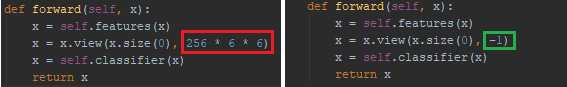
\includegraphics{fig/mistake}
	\caption{On remarque dans la partie de gauche que le code original assume une taille fixe pour la dernière couche de convolution. En plus de limiter le modèle à une certaine taille d'image en entrée on ne peut réduire la dernière couche de convolution. La solution proposée demande la modification dans le section de droite de l'image qui permet une taille variable de la dernière couche de convolution.}
	\label{fig:mistake}
\end{figure}


\subsection{Propagation de l’effet}
Lorsque nous retirons un filtre de convolution d’une couche, il faut prendre plusieurs précautions pour assurer la stabilité du système. Par exemple, il faut ajuster les poids, le nombre de biais dans la couche et ajuster les gradients lorsque ces derniers sont contenus dans la couche elle-même. Ce qui est le cas de PyTorch.

Par la suite, il faut ajuster les couches suivantes en fonction de leur type.
\begin{itemize}[noitemsep, noitemsep, label={}]
	\item Pour les couches de \textbf{convolutions suivantes}. Il est nécessaire d’ajuster le nombre de filtres en entrées pour concorder avec la couche de convolution que nous traitons. Il faut aussi ajuster les poids de cette couche. 
	\item Pour les couches de \textbf{Batchnorm}, il faut ajuster les biais lorsqu'ils sont utilisés et nous effectuons un reset sur les variables utilisées à l’exécution. Dans PyTorch, nous parlons de running means et running vars. 
	\item Finalement, nous devons ajuster les couches \textbf{pleinement connectées}. Dans le cas de ces couches, nous ajustons les poids et nous appliquons la \textit{weight inference rule}\cite{weightinference} afin de simuler le retrait des poids par \textit{dropout}. 
\end{itemize}

Les autres couches semblent bien supporter la réduction de couches de convolution. Il est à noter que nous avons uniquement essayé les modèles proposés dans PyTorch et que plus de travail pourrait être nécessaire pour des couches plus complexes. 
\newpage
\subsection{Description des paramètres}
Afin d'obtenir les résultat présentés. Les tests ont été fait sur l'ensemble de données CIFAR10 et les poids pré entrainé de PyTorch ont été utilisé. La seule transformation appliquée aux images a été d'appliqué une normalization avec moyenne de [0.485, 0.456, 0.406] et une déviation standard de [0.229, 0.224, 0.225].
L'optimiseur utilisé était SGD, sans momentum, ni utilisation de Nesterov. Ainsi qu'un learning rate constant de 0.01.

\section*{Résultats}
Dans un premier temps, nous évaluons l’effet de la réduction des filtres de convolution sur le modèle AlexNet. La figure 3 montre les effets de la réduction.
\begin{figure}[H]
	\centering
	\begin{subfigure}[b]{0.33\textwidth}            
		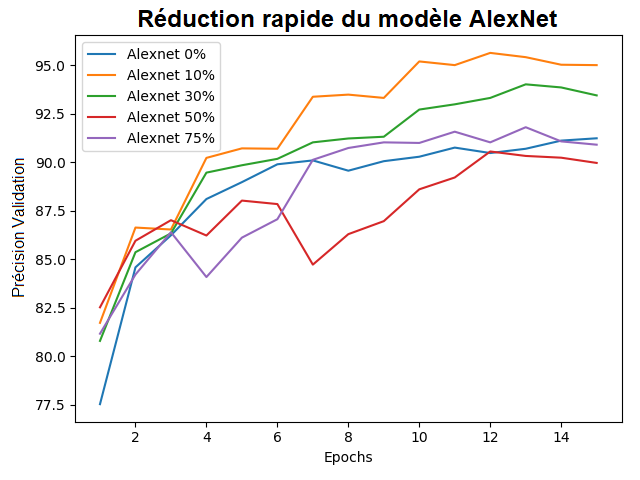
\includegraphics[width=\textwidth]{fig/prune_ratio_rough_fr}
		\label{fig:pruneratiorough}
	\end{subfigure}%
	%add desired spacing between images, e. g. ~, \quad, \qquad etc.
	%(or a blank line to force the subfigure onto a new line)
	\begin{subfigure}[b]{0.33\textwidth}
		\centering
		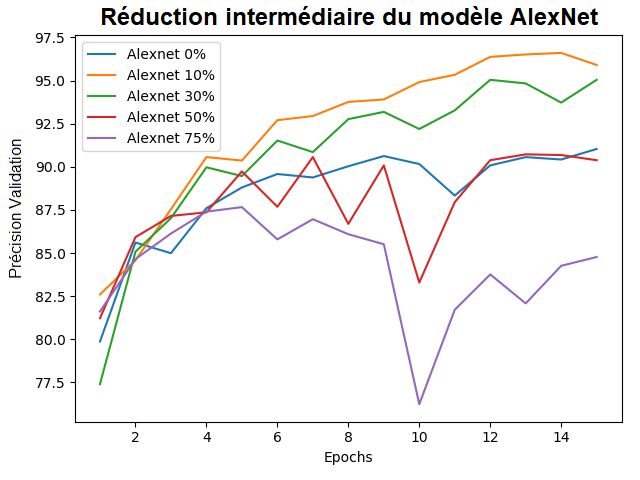
\includegraphics[width=\textwidth]{fig/prune_ratio_medium_fr}
		\label{fig:pruneratioslow}
	\end{subfigure}
	\begin{subfigure}[b]{0.33\textwidth}
		\centering
		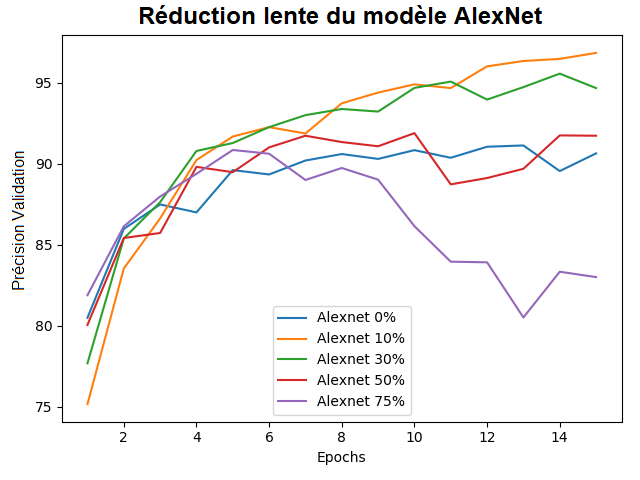
\includegraphics[width=\textwidth]{fig/prune_ratio_slow_fr}
		\label{fig:pruneratioslow}
	\end{subfigure}
	\caption{Dans la figure de gauche, on constate une réduction importante des poids à chaque itération(epoch 4 et 7). La figure du centre représente une réduction sur 4 itérations avec 2 étapes de remise à niveau. Sur la figure de droite, on voit une réduction plus progressive faite sur 10 itérations.}
\end{figure}

\begin{table}[H]
	\centering
	\caption {\textbf{Comparaison des résultats après la réduction des modèles}}
	\begin{tabular}{clllll}
		\textbf{}                & \multicolumn{1}{c}{\textbf{0\%}} & \multicolumn{1}{c}{\textbf{10\%}} & \multicolumn{1}{c}{\textbf{30\%}} & \multicolumn{1}{c}{\textbf{50\%}} & \multicolumn{1}{c}{\textbf{75\%}} \\
		\textbf{Fast Pruning}    & 91.02                            & 88.94                             & 89.94                             & 88.01                             & 88.79                             \\
		\textbf{Average Pruning} & 90.78                            & 90.85                             & 90.39                             & 87.17                             & 83.58                             \\
		\textbf{Slow Pruning}    & 90.74                            & 90.14                             & 89.43                             & 87.84                             & 81.02                            
	\end{tabular}
\end{table}
\newpage
La figure 3 montre un aspect important. Nous remarquons que la manière de réduire les poids est importante. Une réduction trop rapide des poids va causer un plus grand bruit dans l'entrainement. Cependant le nombre d'epochs d'entrainement effectué après la dernière réduction semble essentiel pour obtenir de bons résultats. À l'opposé, nous remarquons qu'une réduction graduelle appliquée sur une plus longue période apporte plus de stabilité dans le modèle pour un certain temps, mais que le nombre d'itérations de réduction finit par réduire les performances finales du modèle. Une approche entre les deux obtient une bonne stabilité dans le modèle et les résultats finaux sont plus consistants.


Par la suite, nous comparons la différence d’efficacité entre les modèles. Cette différence est visible dans la figure 4 qui compare les modèles peu profonds dans la section de gauche et les modèles profonds de Pytorch dans le graphique de droite. Dans tous les cas, on remarque que même avec une réduction de 30\%. Il est possible de réduire significativement le réseau et maintenir un niveau de performance.

\begin{figure}[H]
	\centering
	\begin{subfigure}[b]{0.5\textwidth}            
		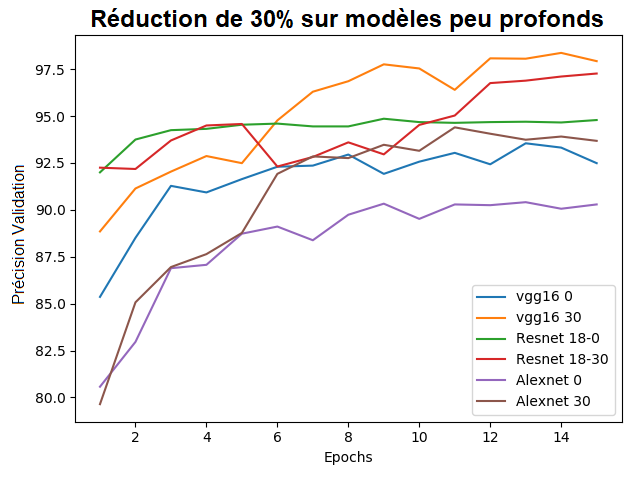
\includegraphics[width=\textwidth]{fig/various_models_shallow_fr}
		\label{fig:SRl}
	\end{subfigure}%
	%add desired spacing between images, e. g. ~, \quad, \qquad etc.
	%(or a blank line to force the subfigure onto a new line)
	\begin{subfigure}[b]{0.5\textwidth}
		\centering
		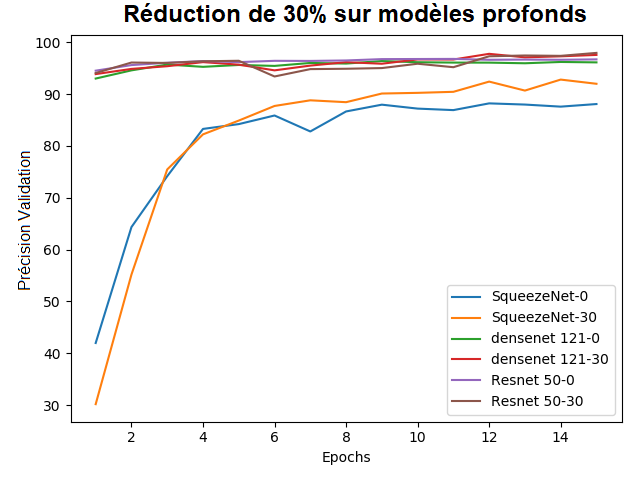
\includegraphics[width=\textwidth]{fig/various_models_deep_fr}
		\label{fig:D-Imager}
	\end{subfigure}
	\caption{Dans l'image de gauche on peut observer l'effet de la réduction sur les modèles peu profonds. Dans l'image de droite on voit l'effet de la réduction sur les réseaux profonds de PyTorch.}
\end{figure}
\newpage
La stratégie utilisée pour la réduction est de faire une réduction progressive. C'est à dire couper 5\% filtres pouvant être réduit et répéter pour 6 itérations. Nous observons que cette stratégie donne de meilleurs résultats sur tous les modèles au niveau de la validation. Cependant on remarque que les score finaux sont légèrement inférieurs dans la majorité des cas.
\begin{table}[H]
	\caption {\textbf{Comparaison de la réduction en fonction du modèle}}
\begin{tabular}{cccccccccc}
	\multicolumn{1}{l}{\textbf{}}           & \multicolumn{3}{c}{\textbf{VGG}}                                                                            & \multicolumn{3}{c}{\textbf{AlexNet}}                                                                        & \multicolumn{3}{c}{\textbf{ResNet18}}                                                                      \\
	\multicolumn{1}{l}{}                    & 0\%                       & 30\%                      & Diff                                                & 0\%                       & 30\%                      & Diff                                                & 0\%                       & 30\%                      & Diff                                               \\ \cline{2-10} 
	\multicolumn{1}{c|}{\textbf{FLOPs (G)}}  & \multicolumn{1}{l}{17.31} & \multicolumn{1}{l}{10.55} & \multicolumn{1}{l|}{{\color[HTML]{009901} -39.1\%}} & \multicolumn{1}{l}{0.815} & \multicolumn{1}{l}{0.500} & \multicolumn{1}{l|}{{\color[HTML]{009901} -38.7\%}} & \multicolumn{1}{l}{1.83}  & \multicolumn{1}{l}{1.40}  & \multicolumn{1}{l}{{\color[HTML]{009901} -23.5\%}} \\
	\multicolumn{1}{c|}{\textbf{Params (M)}} & \multicolumn{1}{l}{138.3} & \multicolumn{1}{l}{80.5}  & \multicolumn{1}{l|}{{\color[HTML]{009901} -42.8\%}} & \multicolumn{1}{l}{57.0}  & \multicolumn{1}{l}{47.9}  & \multicolumn{1}{l|}{{\color[HTML]{009901} -16.0\%}} & \multicolumn{1}{l}{11.18} & \multicolumn{1}{l}{7.53}  & \multicolumn{1}{l}{{\color[HTML]{009901} -32.6\%}} \\
	\multicolumn{1}{l|}{\textbf{Score (\%)}} & \multicolumn{1}{l}{91.92} & \multicolumn{1}{l}{92.03} & \multicolumn{1}{l|}{{\color[HTML]{009901} 0.11}}    & \multicolumn{1}{l}{90.98} & \multicolumn{1}{l}{88.57} & \multicolumn{1}{l|}{{\color[HTML]{9A0000} -2.41}}   & \multicolumn{1}{l}{94.8}  & \multicolumn{1}{l}{93.11} & \multicolumn{1}{l}{{\color[HTML]{9A0000} -1.69}}   \\ \hline
	\multicolumn{1}{l}{}                    & \multicolumn{1}{l}{}      & \multicolumn{1}{l}{}      & \multicolumn{1}{l}{}                                & \multicolumn{1}{l}{}      & \multicolumn{1}{l}{}      & \multicolumn{1}{l}{}                                & \multicolumn{1}{l}{}      & \multicolumn{1}{l}{}      & \multicolumn{1}{l}{}                               \\
	& \multicolumn{3}{c}{\textbf{SqueezeNet}}                                                                     & \multicolumn{3}{c}{\textbf{DenseNet121}}                                                                    & \multicolumn{3}{c}{\textbf{ResNet50}}                                                                      \\
	& 0\%                       & 30\%                      & Diff                                                & 0\%                       & 30\%                      & Diff                                                & 0\%                       & 30\%                      & Diff                                               \\ \cline{2-10} 
	\multicolumn{1}{c|}{\textbf{FLOPs (G)}}  & 0.516                     & 0.511                     & \multicolumn{1}{c|}{{\color[HTML]{009901} -0.97\%}} & 2.91                      & 2.14                      & \multicolumn{1}{c|}{{\color[HTML]{009901} -26.4\%}} & 4.14                      & 2.86                      & {\color[HTML]{009901} -30.9\%}                     \\
	\multicolumn{1}{c|}{\textbf{Params (M)}} & 1.24                      & 1.23                      & \multicolumn{1}{c|}{{\color[HTML]{009901} -0.81\%}} & 7.98                      & 6.12                      & \multicolumn{1}{c|}{{\color[HTML]{009901} -23.3\%}} & 23.53                     & 11.18                     & {\color[HTML]{009901} -52.5\%}                     \\
	\multicolumn{1}{c|}{\textbf{Score (\%)}} & 88.22                     & 88.87                     & \multicolumn{1}{c|}{{\color[HTML]{009901} 0.65}}    & 95.99                     & 95.31                     & \multicolumn{1}{c|}{{\color[HTML]{9A0000} -0.68}}   & 96.32                     & 94.76                     & {\color[HTML]{9A0000} -1.56}                      
\end{tabular}
\end{table}

En examinant l’effet de la réduction sur les paramètres et le nombre de FLOPs dans la table1.  Nous remarquons qu'une réduction de 30\% des filtres disponibles varie grandement d’un modèle à l’autre. Par exemple, dans SqueezeNet, il n’y a que la première couche de convolution qui peut être réduite. Ce qui explique une aussi petite réduction. À l’opposé, les réseaux du type ResNet offrent une excellente réduction, mais ont une dégradation de leur performance. 

La perte ne semble pas directement relié au pourcentage de paramètres ou le nombre d'opérations flottantes retirés du réseau. Pour une réduction similaire VGG n'a aucune dégradation alors que ResNet18 montre une perte de 1.69\%.

\section*{Conclusion}
En conclusion nous remarquons: 1- La technique de réduction des filtres de convolution peut être appliqués sur des modèles plus complexes en créant un module analysant l’exécution du modèle. 2 - Les gains en réduction peuvent permettre de réduire les besoins matériels pour beaucoup d’architectures. 3 - La réduction de filtres de convolution offre une forme de régularisation pouvant servir à l’entrainement d'un modèle lorsque appliqué modérément. 4 - La manière d’appliquer la réduction est important afin d'obtenir de bons résultats. 5 - Certains modèles offrent très peu de réduction. 6 - Il reste du travail afin de supporter adéquatement les optimiseurs.

\newpage
\bibliography{scibib}

\bibliographystyle{Science}


\end{document}
